% Options for packages loaded elsewhere
\PassOptionsToPackage{unicode}{hyperref}
\PassOptionsToPackage{hyphens}{url}
%
\documentclass[
]{article}
\usepackage{lmodern}
\usepackage{amssymb,amsmath}
\usepackage{ifxetex,ifluatex}
\ifnum 0\ifxetex 1\fi\ifluatex 1\fi=0 % if pdftex
  \usepackage[T1]{fontenc}
  \usepackage[utf8]{inputenc}
  \usepackage{textcomp} % provide euro and other symbols
\else % if luatex or xetex
  \usepackage{unicode-math}
  \defaultfontfeatures{Scale=MatchLowercase}
  \defaultfontfeatures[\rmfamily]{Ligatures=TeX,Scale=1}
\fi
% Use upquote if available, for straight quotes in verbatim environments
\IfFileExists{upquote.sty}{\usepackage{upquote}}{}
\IfFileExists{microtype.sty}{% use microtype if available
  \usepackage[]{microtype}
  \UseMicrotypeSet[protrusion]{basicmath} % disable protrusion for tt fonts
}{}
\makeatletter
\@ifundefined{KOMAClassName}{% if non-KOMA class
  \IfFileExists{parskip.sty}{%
    \usepackage{parskip}
  }{% else
    \setlength{\parindent}{0pt}
    \setlength{\parskip}{6pt plus 2pt minus 1pt}}
}{% if KOMA class
  \KOMAoptions{parskip=half}}
\makeatother
\usepackage{xcolor}
\IfFileExists{xurl.sty}{\usepackage{xurl}}{} % add URL line breaks if available
\IfFileExists{bookmark.sty}{\usepackage{bookmark}}{\usepackage{hyperref}}
\hypersetup{
  pdftitle={Changes in sentiment of US federal fisheries regulations during COVID-19},
  pdfauthor={Gavin Fay1,; Scott I. Large2},
  pdfkeywords={COVID-19; management complexity; sentiment},
  hidelinks,
  pdfcreator={LaTeX via pandoc}}
\urlstyle{same} % disable monospaced font for URLs
\usepackage[margin=1in]{geometry}
\usepackage{longtable,booktabs}
% Correct order of tables after \paragraph or \subparagraph
\usepackage{etoolbox}
\makeatletter
\patchcmd\longtable{\par}{\if@noskipsec\mbox{}\fi\par}{}{}
\makeatother
% Allow footnotes in longtable head/foot
\IfFileExists{footnotehyper.sty}{\usepackage{footnotehyper}}{\usepackage{footnote}}
\makesavenoteenv{longtable}
\usepackage{graphicx,grffile}
\makeatletter
\def\maxwidth{\ifdim\Gin@nat@width>\linewidth\linewidth\else\Gin@nat@width\fi}
\def\maxheight{\ifdim\Gin@nat@height>\textheight\textheight\else\Gin@nat@height\fi}
\makeatother
% Scale images if necessary, so that they will not overflow the page
% margins by default, and it is still possible to overwrite the defaults
% using explicit options in \includegraphics[width, height, ...]{}
\setkeys{Gin}{width=\maxwidth,height=\maxheight,keepaspectratio}
% Set default figure placement to htbp
\makeatletter
\def\fps@figure{htbp}
\makeatother
\setlength{\emergencystretch}{3em} % prevent overfull lines
\providecommand{\tightlist}{%
  \setlength{\itemsep}{0pt}\setlength{\parskip}{0pt}}
\setcounter{secnumdepth}{5}

\title{Changes in sentiment of US federal fisheries regulations during COVID-19}
\author{Gavin Fay\textsuperscript{1,*} \and Scott I. Large\textsuperscript{2}}
\date{09 June, 2020}

\begin{document}
\maketitle
\begin{abstract}
The COVID-19 crisis has had a significant impact on the US seafood industry, with disruption to both fishing activity and distribution of products to markets, particularly with restaurant closures. Reductions in fishing activity have been concomitant with efforts by fishers and supporting organizations to pivot to alternative markets and new initiatives to sell and distribute products. In addition, both state and federal fisheries regulators and management agencies have made changes to rules that affect fishing behavior, including monitoring requirements and shifts in governing when, where, and what fishers can catch. A strategic goal of fisheries management in the US is to reduce burdens of regulatory complexity on fishers, as a means of promoting increased production from wild capture fisheries. Here we perform sentiment analysis of US federal fisheries rules published in the Code of Federal Regulations to assess whether recent rule changes during the COVID-19 crisis have used language suggestive of relaxing constraints on fishers (e.g.~easing regulations), and compare changes in rules sentiment to those observed during other recent large-scale shocks to the US seafood system. Finally, we evaluate changes in US fisheries regulation texts in the context of changes within the entire US Federal Register system.
\end{abstract}

{
\setcounter{tocdepth}{2}
\tableofcontents
}
\textsuperscript{1} Department of Fisheries Oceanography, School for Marine Science and Technology, University of Massachusetts Dartmouth, New Bedford, MA 02744, USA\\
\textsuperscript{2} NOAA Fisheries Northeast Fisheries Science Center, Woods Hole, MA 02543, USA

\textsuperscript{*} Correspondence: \href{mailto:gfay@umassd.edu}{Gavin Fay \textless{}\href{mailto:gfay@umassd.edu}{\nolinkurl{gfay@umassd.edu}}\textgreater{}}

Keywords: COVID-19; management complexity; sentiment

Highlights: These are the highlights.

\hypertarget{introduction}{%
\section{Introduction}\label{introduction}}

Here is a citation (Marwick, 2017)
The COVID-19 crisis has had a significant impact on the seafood industry, with closures and restrictions to both fishing activity and distribution of seafood products to markets creating a large shock to the seafood supply chain. These impacts affect both fishers and also other businesses that are part of the seafood supply chain in and around working waterfronts and coastal communities.

In concert and in response to these changes, US fisheries have seen both large scale and regional changes to regulations, including designation of CARES act funding, chiefly aimed at providing relief to fishers, to reduce restrictions on fishing activity, and also to promote workforce safety, notably the waiver of observer requirements because of risks associated with COVID-19 spread.
Text here supporting claims about changes in regulations

As NOAA Fisheries moves toward implementing Integrated Ecosystem Approaches to management, require systemic indicators across both strategic and tactical objectives.
Indicators for governance system
Strategic plans (and EO) calls for reducing regulatory burdens on fisheries
How to quantify these?

Here we perform sentiment analysis of US federal fisheries rules published in the code of federal regulations to assess whether recent rule changes during the COVID-19 crisis have used language suggestive of relaxing constraints on fishers (e.g.~easing regulations), and compare changes in rules sentiment to those observed during other recent large-scale shocks to the US seafood system (implementation of catch shares). Finally, we evaluate changes in US fisheries regulation texts in the context of changes within the entire US federal registry system

\hypertarget{methods}{%
\section{Methods}\label{methods}}

\hypertarget{data}{%
\subsection{Data}\label{data}}

Table \ref{tab:cfr-part-table})

\begin{itemize}
\item
  Subpart (e.g., Groundfish plan)
\item
  Body to evaluate

  \begin{itemize}
  \tightlist
  \item
    FR - actions, summary of regulations (abstract), most recent action, \# of pages
  \item
    CFR - (eCFR)
  \end{itemize}
\item
  Implementation of catch shares created a more restrictive/ volume set of rules
\item
  Sentiment analysis - trends in \#s
\item
  What words are correlating with sentiment score (reduce, waive, relax, extension)

  \begin{itemize}
  \tightlist
  \item
    Think about what exactly we want to measure.
  \end{itemize}
\item ~
  \hypertarget{pages-as-proxy-of-complexity-sentiment-analysis-on-summary-on-whole-regulation}{%
  \section{pages as proxy of complexity, sentiment analysis on summary \& on whole regulation}\label{pages-as-proxy-of-complexity-sentiment-analysis-on-summary-on-whole-regulation}}
\item
  Compare effect relative to catch shares (or ACLs)
\item
  Resampling distributions
\end{itemize}

\begin{table}

\caption{\label{tab:cfr-part-table}Title 50---Wildlife and Fisheries\nCHAPTER VI--Fishery Conservation and Management, National Oceanic and Atmospheric Administration, Department of Commerce}
\centering
\begin{tabular}[t]{r|l}
\hline
Part & Name\\
\hline
600 & Magnuson-Stevens Act Provisions\\
\hline
622 & Fisheries of the Caribbean, Gulf of Mexico, and South Atlantic\\
\hline
635 & Atlantic Highly Migratory Species\\
\hline
648 & Fisheries of the Northeastern United States\\
\hline
660 & Fisheries Off West Coast States\\
\hline
665 & Fisheries in the Western Pacific\\
\hline
679 & Fisheries of the Exclusive Economic Zone Off Alaska\\
\hline
680 & Shellfish Fisheries of the Exclusive Economic Zone Off Alaska\\
\hline
697 & Atlantic Coastal Fisheries Cooperative Management\\
\hline
\end{tabular}
\end{table}

\hypertarget{results}{%
\section{Results}\label{results}}

\begin{itemize}
\tightlist
\item
  General trend in \#s of regulations, \#of pages.
\item
  Sentiment of rules in 2020 compared to other years

  \begin{itemize}
  \tightlist
  \item
    Split by part \& subpart
  \item
    Linear model to aid interpretation
  \end{itemize}
\item
  Comparison to catch share, at same resolution
\item
  Comparison to resample distribution for random parts \& subparts
\end{itemize}

\begin{figure}
\centering
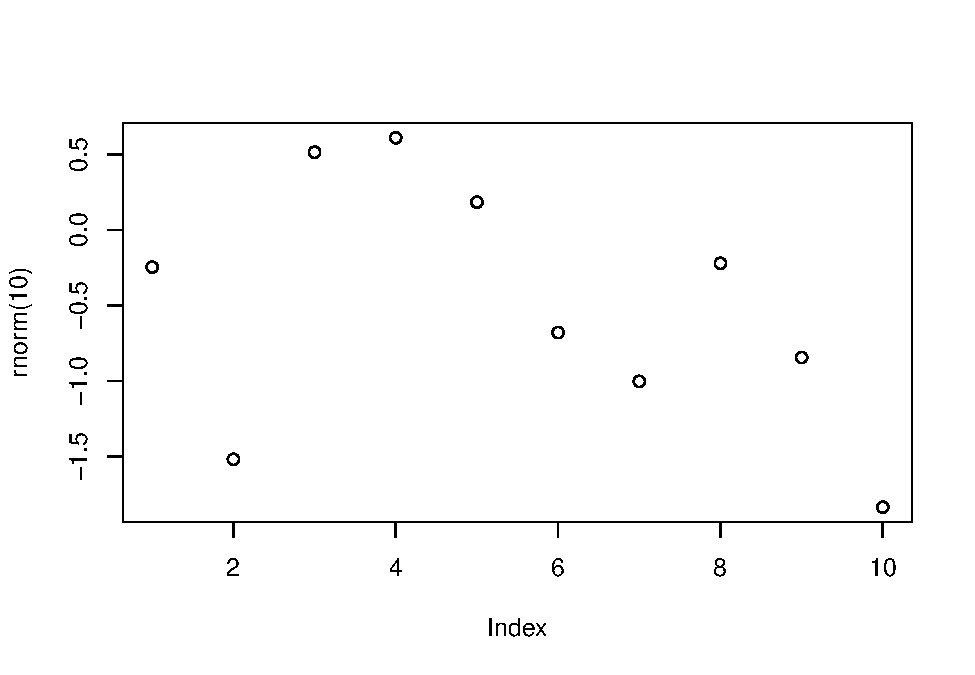
\includegraphics{../figures/demo-plot-1.pdf}
\caption{\label{fig:demo-plot}A plot of random numbers}
\end{figure}

Figure \ref{fig:demo-plot} shows how we can have a caption and cross-reference for a plot

Here is an example of inline code 3.14 in the middle of a sentence.

\hypertarget{discussion}{%
\section{Discussion}\label{discussion}}

\hypertarget{conclusion}{%
\section{Conclusion}\label{conclusion}}

\hypertarget{acknowledgements}{%
\section{Acknowledgements}\label{acknowledgements}}

\newpage

\hypertarget{references}{%
\section{References}\label{references}}

\hypertarget{refs}{}
\leavevmode\hypertarget{ref-Marwick2017}{}%
Marwick, B., 2017. Computational reproducibility in archaeological research: Basic principles and a case study of their implementation. Journal of Archaeological Method and Theory 24, 424--450. \url{https://doi.org/10.1007/s10816-015-9272-9}

\newpage

\hypertarget{colophon}{%
\subsubsection{Colophon}\label{colophon}}

This report was generated on 2020-06-09 13:29:13 using the following computational environment and dependencies:

\begin{verbatim}
#> - Session info ---------------------------------------------------------------
#>  setting  value                       
#>  version  R version 3.6.1 (2019-07-05)
#>  os       Windows 10 x64              
#>  system   x86_64, mingw32             
#>  ui       RTerm                       
#>  language (EN)                        
#>  collate  English_United States.1252  
#>  ctype    English_United States.1252  
#>  tz       America/New_York            
#>  date     2020-06-09                  
#> 
#> - Packages -------------------------------------------------------------------
#>  package     * version    date       lib source                         
#>  assertthat    0.2.1      2019-03-21 [1] CRAN (R 3.6.1)                 
#>  backports     1.1.5      2019-10-02 [1] CRAN (R 3.6.1)                 
#>  bookdown      0.18       2020-03-05 [1] CRAN (R 3.6.3)                 
#>  callr         3.4.3      2020-03-28 [1] CRAN (R 3.6.3)                 
#>  cli           2.0.2      2020-02-28 [1] CRAN (R 3.6.3)                 
#>  crayon        1.3.4      2017-09-16 [1] CRAN (R 3.6.1)                 
#>  desc          1.2.0      2018-05-01 [1] CRAN (R 3.6.1)                 
#>  devtools      2.2.2.9000 2020-03-30 [1] Github (r-lib/devtools@f77c14e)
#>  digest        0.6.25     2020-02-23 [1] CRAN (R 3.6.3)                 
#>  ellipsis      0.3.0      2019-09-20 [1] CRAN (R 3.6.3)                 
#>  evaluate      0.14       2019-05-28 [1] CRAN (R 3.6.1)                 
#>  fansi         0.4.1      2020-01-08 [1] CRAN (R 3.6.3)                 
#>  fs            1.3.2      2020-03-05 [1] CRAN (R 3.6.3)                 
#>  glue          1.3.2      2020-03-12 [1] CRAN (R 3.6.3)                 
#>  highr         0.8        2019-03-20 [1] CRAN (R 3.6.1)                 
#>  htmltools     0.4.0      2019-10-04 [1] CRAN (R 3.6.3)                 
#>  knitr         1.28       2020-02-06 [1] CRAN (R 3.6.3)                 
#>  magrittr      1.5        2014-11-22 [1] CRAN (R 3.6.1)                 
#>  memoise       1.1.0      2017-04-21 [1] CRAN (R 3.6.1)                 
#>  pkgbuild      1.0.6      2019-10-09 [1] CRAN (R 3.6.3)                 
#>  pkgload       1.0.2      2018-10-29 [1] CRAN (R 3.6.1)                 
#>  prettyunits   1.1.1      2020-01-24 [1] CRAN (R 3.6.3)                 
#>  processx      3.4.2      2020-02-09 [1] CRAN (R 3.6.3)                 
#>  ps            1.3.2      2020-02-13 [1] CRAN (R 3.6.3)                 
#>  R6            2.4.1      2019-11-12 [1] CRAN (R 3.6.3)                 
#>  Rcpp          1.0.4      2020-03-17 [1] CRAN (R 3.6.3)                 
#>  remotes       2.1.1      2020-02-15 [1] CRAN (R 3.6.3)                 
#>  rlang         0.4.6      2020-05-02 [1] CRAN (R 3.6.3)                 
#>  rmarkdown     2.1        2020-01-20 [1] CRAN (R 3.6.3)                 
#>  rprojroot     1.3-2      2018-01-03 [1] CRAN (R 3.6.1)                 
#>  sessioninfo   1.1.1      2018-11-05 [1] CRAN (R 3.6.1)                 
#>  stringi       1.4.6      2020-02-17 [1] CRAN (R 3.6.2)                 
#>  stringr       1.4.0      2019-02-10 [1] CRAN (R 3.6.1)                 
#>  testthat      2.3.2      2020-03-02 [1] CRAN (R 3.6.3)                 
#>  usethis       1.6.1      2020-04-29 [1] CRAN (R 3.6.3)                 
#>  withr         2.1.2      2018-03-15 [1] CRAN (R 3.6.1)                 
#>  xfun          0.12       2020-01-13 [1] CRAN (R 3.6.3)                 
#>  yaml          2.2.1      2020-02-01 [1] CRAN (R 3.6.2)                 
#> 
#> [1] C:/Users/scott.large/Documents/R/win-library/3.6
#> [2] C:/Program Files/R/R-3.6.1/library
\end{verbatim}

The current Git commit details are:

\end{document}
